\documentclass[tikz]{standalone}

% Required packages
\usepackage{tikz}
\usetikzlibrary{positioning} % for node distance
\usepackage{graphicx}        % for including images

\begin{document}

\begin{tikzpicture}[
    node distance=4cm, % Default spacing between blocks
    thick,             % Line thickness
    block1/.style={draw, minimum width=2.5cm, minimum height=1.5cm, align=center, rounded corners}, % block1: with border
    block2/.style={minimum width=2.5cm, minimum height=1.5cm, align=center} % block2: without border
]

% Define blocks with styles
\node[block1] (A) {\textbf{Sistema}\\ \textbf{Relazionale}\\ \textbf{Empirico}}; 

\node[block1, right of=A, xshift=2cm] (B) {\textbf{Sistema}\\ \textbf{Relazionale}\\ \textbf{Numerico}}; 

% Draw double arrow
\draw[<->, thick] (A) -- (B);

% Add image below node A
\node[below=0.5cm of A] (A_image) {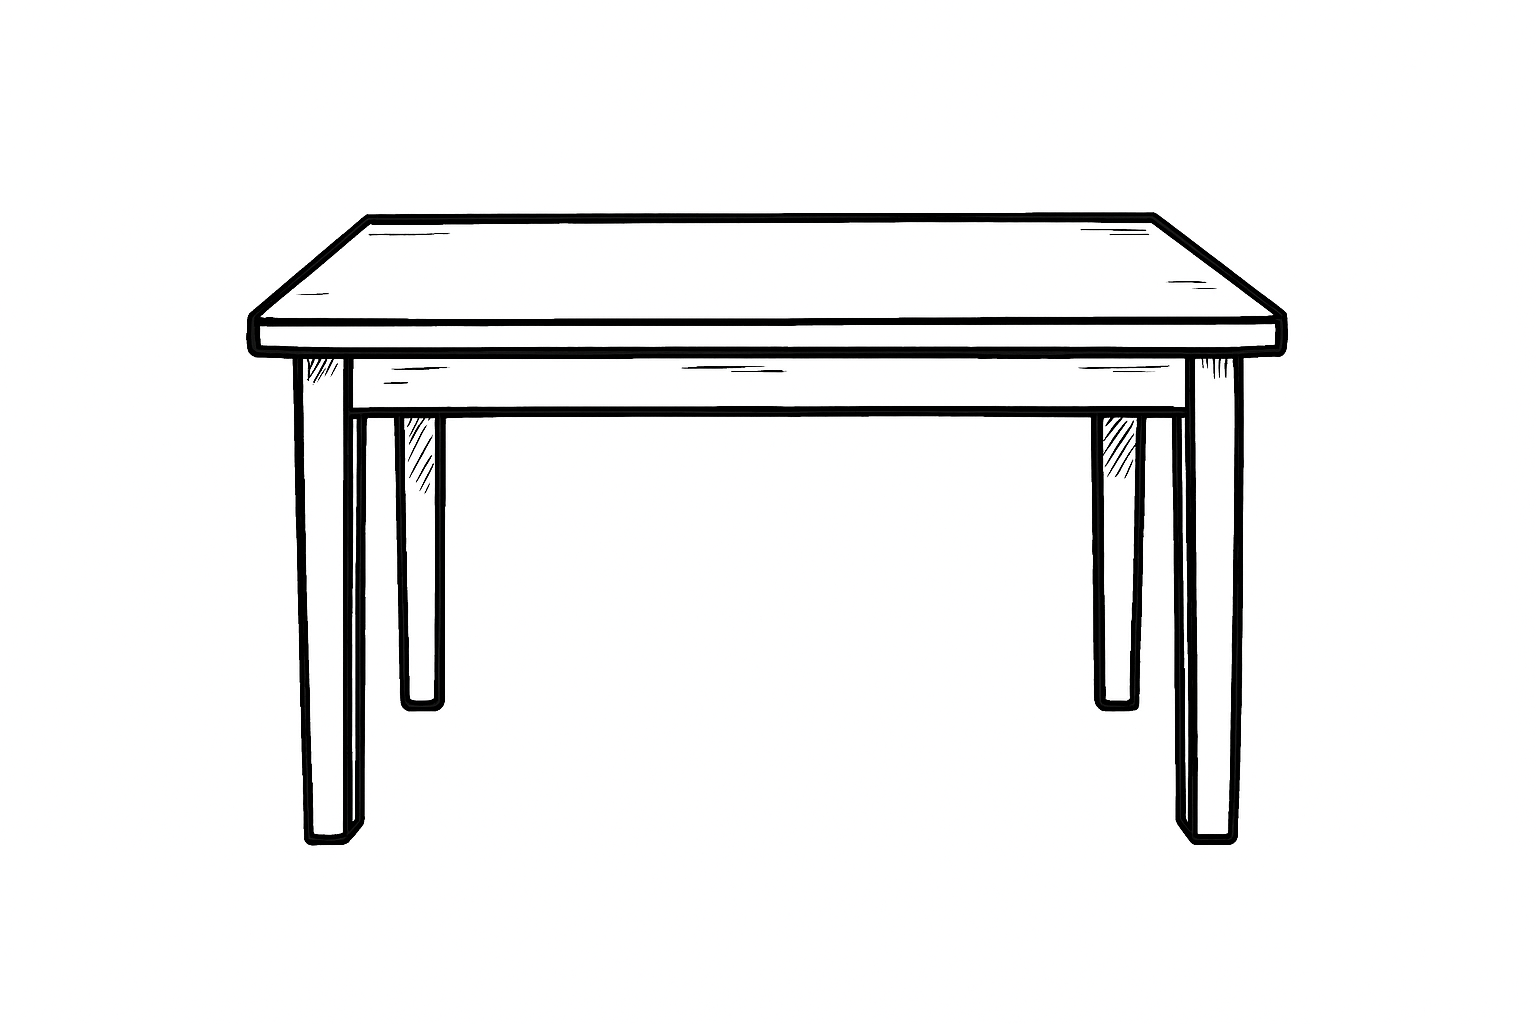
\includegraphics[width=2.5cm]{Table.png}}; 

% Add label below node B
\node[below=1cm of B] (B_label) {120};

\end{tikzpicture}

\end{document}
